% !TEX root = ../SU2-Scitech15.tex

\section{Results}
First executive summary of the results a table and couple figures that show everyone we varied and did. For instance a figure could look like this \cref{fig:Cd_convergence}
Second, organize results subsections either by grid or angle of attack, whichever makes more sense once we have the results.
Third, show validation results for a representative case.
Figures and tables in this section should address questions such as: how do variation in the forces due to changing grids compare with changing the parameters? Which parameters change speed of convergence? Which parameters change value to which we converge? ...

\begin{figure}
  \centering
  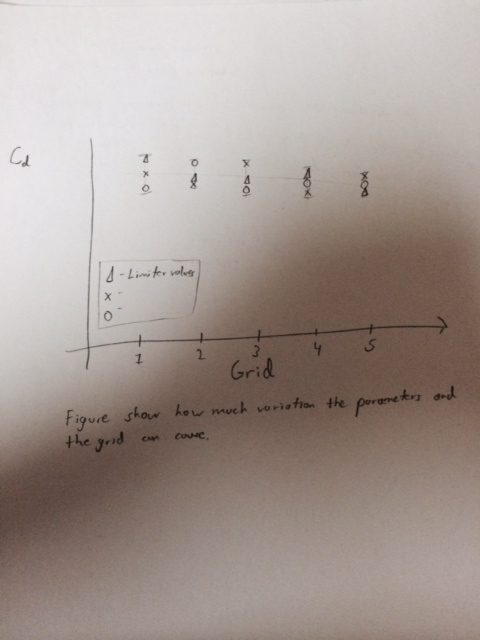
\includegraphics[width=0.5\textwidth]{./fig/cd_convergence}
  \caption{Drag coefficient convergence and variation.}
  \label{fig:Cd_convergence}
\end{figure}

Also, a sample table \cref{tab:sample_table} to be used as a template.

